\documentclass[linenumbers,twocolumn]{aastex62}
\usepackage{enumitem}
%\usepackage{courier}
\graphicspath{{./}{figures/}}
\usepackage[T1]{fontenc}
\usepackage{epsfig}
\usepackage{epstopdf}
\epstopdfsetup{update}
\usepackage{natbib}
\usepackage{amssymb}
\usepackage{amsbsy}
\usepackage{natbib}
\usepackage{subfigure}
\usepackage[mathcal]{euscript}
\usepackage{float}
\usepackage{amsmath}
\usepackage{tabularx}
\usepackage{xspace}
\usepackage{enumitem}
\usepackage{xcolor}
\usepackage{comment}
%\usepackage{appendix}

\newcommand{\blu}{\textcolor{blue} }
\newcommand{\red}{\textcolor{red} }
\newcommand{\grn}{\textcolor{green} }
\newcommand{\cya}{\textcolor{cyan} }
\newcommand{\pink}{\textcolor{magenta} }


\usepackage{ulem,xspace}
\newcommand{\paul}[1]{\textbf{\textcolor{blue}{#1}}}

\newcommand{\crossed}[1]{\red{\xout{#1}}} %querdurchgestrichen
\newcommand{\comment}[1]{{\red{[#1]}}}
\newcommand{\change}[2]{\crossed{#1} \paul{#2}} %crosses out old text and adds text suggested as replacement
\newcommand{\changeC}[3]{\crossed{#1} \paul{#2} \textit{\red{[#3]}}}
\newcommand{\commentR}[2]{\textbf{\textcolor{blue}{#1}} \textit{\red{[#2]}}}
\newcommand{\commentU}[2]{\pink{\uwave{#1}} \textit{\red{[#2]}}}


%\newcommand{\paul}[1]{{\blu{#1}}}
\newcommand{\DP}{$\Delta P$\xspace}
\newcommand{\DPi}{$\Delta \Pi_1$\xspace}
\newcommand{\kms}{km~s$^{-1}$}
\newcommand{\vsini}{\ensuremath{v \sin{i}}}
%\newcommand{\msun}{M$_\sun$}
\newcommand{\tess}{{\it TESS}}
\newcommand{\corot}{{\it CoRoT}}
\newcommand{\jwst}{{\it JWST}}
\newcommand{\kepler}{{\it Kepler}}
\newcommand{\ktwo}{{\it K2}}
\newcommand{\hst}{{\it HST}}
\newcommand{\msun}{$M_{\odot}$}
\newcommand{\rsun}{$R_{\odot}$}
\newcommand{\lsun}{$L_{\odot}$}
\newcommand{\re}{$R_{\oplus}$}
\newcommand{\me}{$M_{\oplus}$}
\newcommand{\rj}{$R_{\textrm{\scriptsize Jup}}$}
\newcommand{\mj}{$M_{\textrm{\scriptsize Jup}}$}
\newcommand{\ms}{m~s$^{-1}$}
\newcommand{\gaia}{\textit{Gaia}}
\newcommand{\spherex}{\textit{SPHEREx}}

\newcommand{\teff}{\mbox{$T_{\rm eff}$}}
\newcommand{\logg}{\mbox{$\log g$}}
\newcommand{\feh}{\mbox{$\rm{[Fe/H]}$}}
\newcommand{\fbol}{\mbox{$f_{\rm bol}$}}
\newcommand{\ctwelvecthirteen}{$^{12}$C/$^{13}$C\xspace}
\newcommand{\hethree}{$^3$He\xspace}

\newcommand{\grad}{\ensuremath{\nabla}}
\newcommand{\gradrad}{\ensuremath{\nabla_{\rm{rad}}}}
\newcommand{\gradad}{\ensuremath{\nabla_{\rm{ad}}}}
\newcommand{\gradmu}{\ensuremath{\nabla_{\mu}}}
\newcommand{\gradL}{\ensuremath{\nabla_{\mathrm{L}}}}
\newcommand{\gradT}{\ensuremath{\nabla_{\mathrm{T}}}}
\newcommand{\brunt}{{Brunt--V\"{a}is\"{a}l\"{a}}}
\newcommand{\Pran}{\ensuremath{\mathrm{Pr}}}
\newcommand{\Dth}{\ensuremath{D_\mathrm{th}}}


%\newcommand{\kiauhoku}{K$\bar{\rm i}$auh$\bar{\rm o}$k$\bar{\rm u}$}
\newcommand{\kiauhoku}{\texttt{kiauhoku}} % I've adopted DFM's practice of using \texttt for software names - zach


\citestyle{aa}
\bibpunct{(}{)}{;}{a}{}{,}

\begin{document}
\title{Empirical Constraints on the Efficiency of Magnetized Thermohaline Mixing}

%\author{Adrian, Matteo, Marc, Meridith, Evan, etc}
\author{Adrian Meridith Evan Jamie}


\author[0000-0002-4818-7885]{Jamie Tayar}
\altaffiliation{NASA Hubble Fellow}
\affiliation{Institute for Astronomy, University of Hawai‘i at Mānoa, 2680 Woodlawn Drive, Honolulu, HI 96822, USA}
\affiliation{Department of Astronomy, University of Florida, Bryant Space Science Center, Stadium Road, Gainesville, FL 32611, USA }


\begin{abstract}
The existence of enhanced extra mixing in low-mass upper giant branch stars has been well documented for decades. It was suggested that their extra mixing might be due to thermohaline convection, which relies on ( mean molecular weight inversions in otherwise stably stratified zones). However, previous attempts to match the observed pattern quantitatively have usually required some sort of ad hoc increase in the efficacy of the thermohaline mixing. Recent simulations have suggested that even moderate magnetic fields could greatly enhance the efficiency of thermhaline mixing, but questions have arisen about the reliability of those predictions given (some simulation limitations). We therefore use the data from the SDSS-IV APOGEE survey of stars covering a range of masses and metallicities to put empirical constraints on the efficiency of mixing as a function of (R0- define) in order to constrain future theoretical investigations. We find that (stuff) and show that this would suggest (cool things).  
\end{abstract}

\keywords{stars: evolution, stars: mixing}

\section{Introduction}
\label{sec:intro}
\setcounter{footnote}{0}
[Begin outline]

\begin{itemize}
    \item In RGB stars there is a first dredge up and then a luminosity bump
    \item Standard models predict no change in surface chemistry after the first dredge up
    \item But observations show extra mixing after the luminosity bump! Explain that, science! [Briefly summarize which observations, which stars, which log g, etc.]
    \item \citet{charbonnel_thermohaline_2007} pointed out it could be thermohaline mixing, this dumb thing that is well-studied in the oceanographic context and had been considered in various other astrophysical settings (see [cite Garaud 2018])
    \item Go into explanation of thermohaline mixing (the stuff that I had previously been writing in the first half of old-section-3, except more of the literature review stuff and less of the mathy/formalism stuff):
    \begin{itemize}
        \item Thermohaline mixing is the mixing of chemicals (heat too but it's a comparably negligible amount) by small-scale turbulent motions that are driven by a double-diffusive instability
        \item Requires a Schwarzschild-stable temperature gradient and an inversion of the $\mu$ profile that is weak enough to still be Ledoux-stable
        \item Also requires thermal diffusion to be larger than chemical diffusion, but this is always the case in stars -- the degree of discrepancy between these diffusion coefficients sets how minimal of a $\mu$ inversion is necessary to trigger thermohaline instability, and in stars this discrepancy is so vast that just about any $\mu$ inversion is immediately unstable
        
        \item The criteria for instability are easy to express in terms of stellar structure variables (see Sec.~\ref{sec:formalism}), making it pretty straightforward to use 1D stellar evolution models to identify where thermohaline mixing could plausibly occur in stars across the HR diagram [list examples]
        
        Because the quantities grad-ad, grad-rad are known at every radial position in a 1D stellar structure model, it is possible to know <values of quantities that are functions of these quantities ($R0$)> at every position. 
        
        \item 
        %But it's much harder to predict what thermohaline mixing actually does to these stars, because 
        historically it's been much more challenging to estimate the efficiency of thermohaline mixing -- just because thermohaline mixing happens doesn't mean it is efficient enough to matter, where matter means?? manifests in surface-observable ways?
        
        \item Summarize efforts to get at efficiency of thermohaline mixing in stellar interiors via analytical theory and multi-dimensional simulations
    \end{itemize}
    \item Arrive at current state of things: a broad range of mixing prescriptions available to MESA users, with 
    %no real clarity
    ongoing literature debate
    as to which model to use, and what values to set for the free parameters
    \item To make matters worse, HG19 shows that magnetic fields of very moderate strengths (plausibly present in majority of these stars) give massively different mixing efficiencies than predictions from hydro theory/3D sims
    \item APOGEE data includes a boat-load of RGB observations -- can we use them to rule out or constrain various thermohaline mixing prescriptions?
    \item Similarly: can observations be used to identify which regions of parameter space simulations should aim to clarify mixing efficiency? (I.e., if two mixing prescriptions agree everywhere except for a certain corner of parameter space, can we use observations to identify whether any stars even live in that parameter space and so whether we should even care?)
    \item In this paper, we present a framework that combines observations and theory to probe the fluid parameters that actually happen in stars
\end{itemize}

[End outline]
%As low-mass stars ascend the red giant branch, their stellar structure is broadly characterized by an inert helium core surrounded by a thin radiation zone, whose inner radii are comprised of the hydrogen burning shell, followed by an extended convective envelope \textcolor{red}{[holy shit what a bad sentence]}.
Standard models of stellar evolution predict that once the convective envelope of a low-mass star \textcolor{red}{[can we be specific about the mass range?]} on the red giant branch has reached its deepest extent, the so called `first dredge up', the surface chemistry of that giant should remain relatively constant through the rest of the shell hydrogen burning phase. 
In contrast, observations of globular cluster \textcolor{red}{[cite?]} as well as low-metallicity field stars \citep{Gratton2000} find significant changes in the abundance ratios of elements known to be sensitive to mixing, including \ctwelvecthirteen, lithium, and [C/N]. 
As the inert helium core grows
These changes seemed to happen only above the red giant branch bump, where the hydrogen burning shell reaches the region where a mean molecular weight gradient was left behind by the deepest evolution of the surface convection zone. These mixing related changes seemed to be largest in the lowest metallicity stars (citecite) and many mechanisms were hard pressed to explain them (cite a bunch of things or maybe a review?). 

\textbf{Adrian:} (enter the theory of thermohaline mixing. mumble mumble ocean. describe how it works. should happen in stars. Helium 3 stuff. maybe not enough citation. maybe magnets? scaling weird. Fraser et al. simulation stuff.  suggest maybe not as efficient? But size and even slope direction of trend unclear analytically/ from simulations. 

One promising mechanism was identified by \citet{charbonnel_thermohaline_2007}: fingering convection, also known as thermohaline mixing. As the hydrogen-burning shell expands into the region that the recent dredge up has rendered chemically homogeneous, the $^3$He($^3$He, 2p)$^4$He reaction creates an inversion of the mean molecular weight $\mu$. While this inverse $\mu$ gradient is not enough to generate a Ledoux-unstable region, it does drive fingering convection. 
%\textcolor{gray}{[OK here's an outline of some stuff that could be said here, but it's probably too much: Briefly summarize instability mechanism but refer readers to Garaud 2018 review. Then talk about Ulrich's model and Kippenhahn's model, which are the most widely used in stellar evolution models but can't be right, especially at large $R_0$ where they predict nontrivial mixing despite the instability shutting off. Mention Denissenkov's fix for this, then the successful Brown 2013 model, both of which have the very physically-reasonable implication that mixing $\to 0$ at large $R_0$. One consequence of these improved models is that thermohaline mixing appears totally insufficient for explaining observations. Bummer. Then \citet{harrington} (hereafter HG19) added magnetic fields to simulations at $R_0 = 1.45$ and $\mathrm{Pm} = 1$ and found dramatic increases in mixing. This is exciting because RGB stars only need magnetic fields on the order of a hundred Gauss to explain observations. Also exciting because (maybe only include this part if I end up publishing this in my in-prep paper) Harrington's model implies these $\mu$ gradients form fully convective layers for certain magnetic field strengths, which can have observational consequences in the AGB stage. Sadly, Fraser \& Garaud have shown that the HG19 model significantly over-predicts mixing when compared to simulations for $\mathrm{Pm} < 1$ -- a ubiquitous feature of these plasmas -- and \textit{especially so for large $R_0$}. While simulations show mixing decreases with decreased $\mathrm{Pm}$ or increased $R_0$, the HG19 model (which does not included $\mathrm{Pm}$ as a parameter but it is readily added) predicts mixing is essentially unaffected by decreased $\mathrm{Pm}$ and can stay constant or even increase as $R_0$ increases. (Maybe also say that it predicts mixing $\to \infty$ as $B_0 \to \infty$ which is unphysical.) However, by necessity due to limitations of computing resources, these simulations only explored $\mathrm{Pr} \sim 10^{-1}$, whereas these regions of RGB stars feature $\mathrm{Pr} \sim 10^{-6}$. Thus, it is unclear if the disagreements between the HG19 model and simulations, especially at large $R_0$, are due to failings of the HG19 model, or due to aspects of thermohaline mixing at $\mathrm{Pr} \sim 10^{-1}$, and thus perhaps the realistic scenario does in fact feature these strange trends in mixing vs $R_0$, but you can only see those trends at really really low $\mathrm{Pr}$. Let's see if we can get an idea via observational constraints!]}

%\textbf{Adrian/Meridith:} Models predict efficiency should scale with R0 (define) (explain why). This can be calculated in 1D simulations (cite Matteo?). in order to compare to theoretical sims. it depends on both He3 abundance and (the other thing). 

%In this paper, we therefore show the possible/proposed dependencies of magnetic thermohaline mixing as a function of R0 in simulations. We use one dimensional stellar evolution models to estimate the range of R0s present in real stars as a function of stellar mass and metallicity, and we use measurements of the amount of mixing in these stars from observations to compare to the predictions of the simulations. 

\section{Observed Mixing Signatures} 
\label{sec:obs}
As discussed in Section \ref{sec:parameterizations}, we are trying to distinguish between different models of thermohaline mixing based not on the amount of mixing they predict, but on their trends as a function of the reduced density ratio $r$. As discussed in Section \ref{sec:mesa_results}, this requires stars of a wide range of masses and metallicities. It is therefore quite convenient that 
modern spectroscopic surveys have recently begun collecting measurements of mixing diagnostics for large samples of stars whose masses are also well constrained. 
%, making it possible to compare observed mixing trends to the predictions of the 
%variety of 
%theoretical models discussed above in Section \ref{sec:parameterizations} by using one dimensional stellar evolution models to estimate the relevant fluid parameters of these stars given their masses and metallicities (Section \ref{sec:mesa_results}). 
%
We choose for this work to use the carbon-to-nitrogen ratios, [C/N], measured from the Apache Point Galactic Evolution Experiment \citep[APOGEE, ][]{Majewski2017}. APOGEE is a Sloan Digital Sky Survey III and IV \citep{Blanton2017} project using the 2.5 meter Sloan Telescope \citep{Gunn2006} and the APOGEE spectrograph \citep{Wilson2019} to obtain medium resolution (R $\sim$ 22,500) spectra of large numbers of stars across the galaxy \citep{Zasowski2017, Beaton2021,Santana2021}. These spectra are homogeneously reduced and analyzed using the ASPCAP pipeline \citep{Nidever2015, Zamora2015, GarciaPerez2016} and the resulting stellar parameters are then calibrated using asteroseismic, cluster, and field data \citep{Holtzman2015,Holtzman2018, Jonsson2020}. We choose to use the APOGEE data because this calibration work has already been done and an asteroseismic overlap sample is already available to provide stars with precise and accurate masses, though %\sout{we acknowledge that} 
similar work could likely be done with, for example, the lithium abundances measured by the GALAH survey \citep{buder2019} or the \ctwelvecthirteen data estimated from the APOGEE data using the Brussels Automatic Code for Characterizing High accUracy Spectra \citep[BACCHUS,][]{Masseron2016_BACCHUS} pipeline (C. Hayes, submitted). 

%FIGURE omgcomp---------------------------------------------------
\begin{figure}[!tb]
\begin{center}
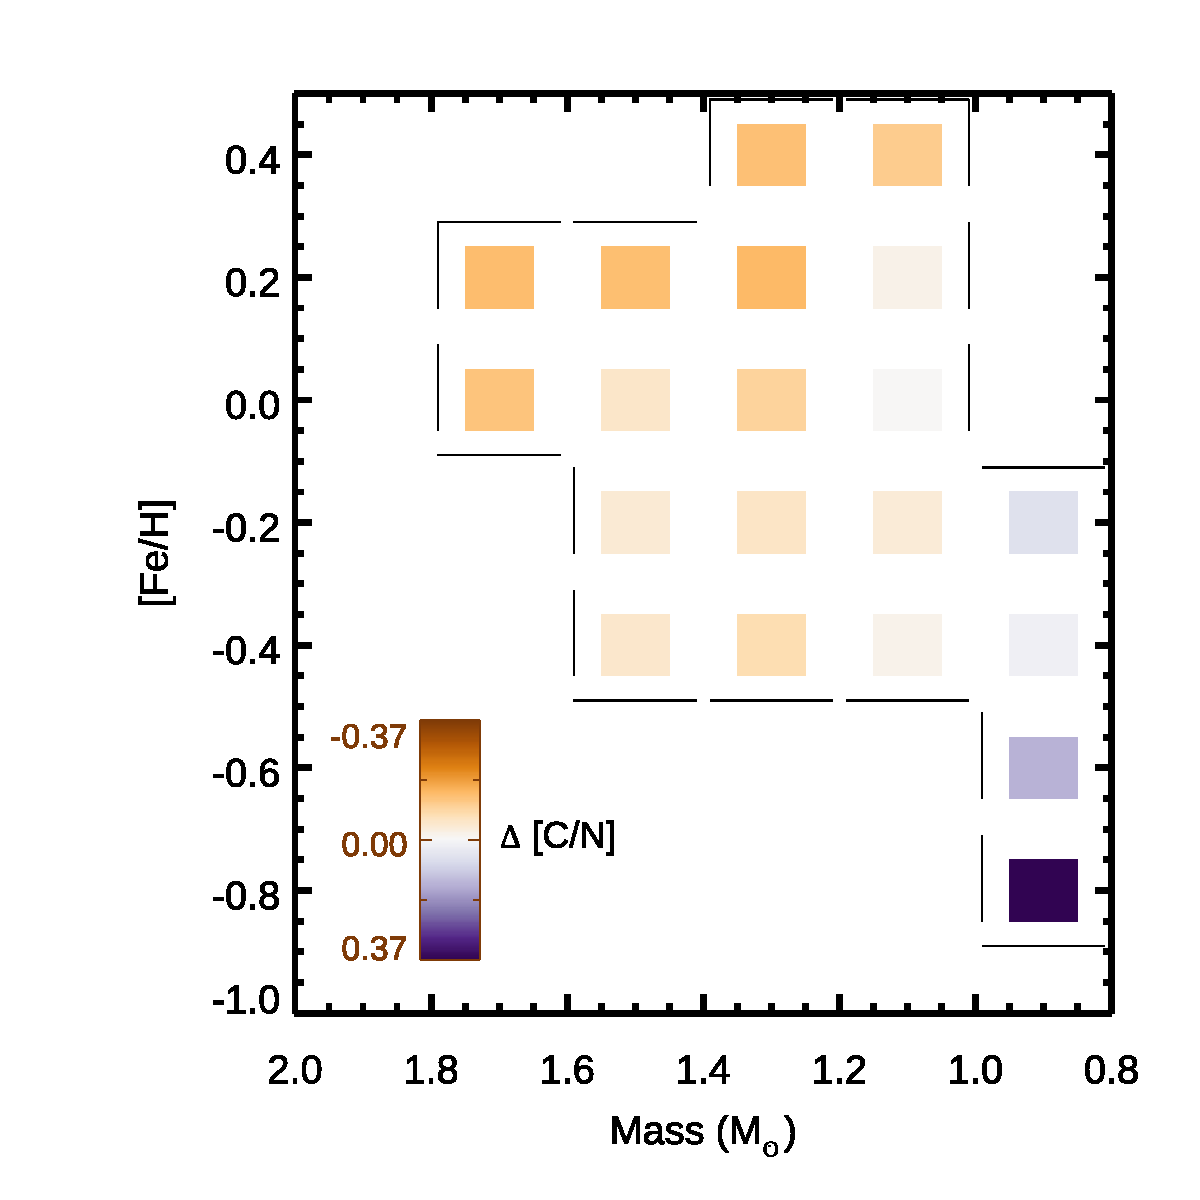
\includegraphics[width=9cm,clip=true, trim=0.5in 0in 0in 0in]{Mfeh5c_mixingCRGBdr14v7.pdf}%[width=9cm, clip=true, trim=1in 1in 1in 1in]{./Figs/omgcomp.eps}
\caption{
The difference in average [C/N] (indicated by box color, with negative values in orange and positive values in purple) between stars significantly below the RGB bump and those significantly above the bump is shown as a function of stellar mass and metallicity. The gradient is consistent with previous work, with lower mass, lower metallicity stars having more extra mixing (purple), but there is clearly an unphysical `unmixing' trend (orange) that needs to be removed (see text). We highlight only bins with a sufficient number of stars both below and above the bump. }
\label{fig:obssquare}
\end{center}
\end{figure}
%FIGURE omgcomp---------------------------------------------------




We also note that the evolution of [C/N] is in some ways simpler for these low-mass stars than other mixing diagnostics. Unlike lithium, its abundance at the surface does not change significantly during the main sequence due to the effects of rotational and other mixing processes \citep{Iben1967}. Its initial ratio seems to be somewhat metallicity dependent \citep{Shetrone2019}, with higher values at lower metallicity. As stars reach the first dredge up, there is a strong, rapid, mass--\textbf{ and metallicity--}dependent change in the surface [C/N] ratio \citep{Salaris2015, MasseronGilmore2015, Martig2016, Ness2016, Spoo2022}. The [C/N] ratio at the surface then remains constant until stars reach the red giant branch bump, after which there seems to be another rapid drop in the [C/N] ratio, particularly in stars of low metallicity \citep[e.g.][]{Gratton2000,Shetrone2019}; it is this drop that has been associated with thermohaline mixing.  For stars of particularly low metallicities, there are some suggestions of Upper RGB extra mixing \citep{Shetrone2019}, but this is not well motivated theoretically and is distinct from the processes we are discussing here.

To estimate the amount of extra mixing in these stars near the bump---which thermohaline models suggest should correlate with the mixing coefficient $\Dth$ described above---\citet{Shetrone2019} estimated the drop in [C/N] just above the red giant branch bump. Their work used $\alpha$-element enhanced, and therefore old and low-mass ($\sim$0.9 \msun), first ascent red giant branch stars and binned them in bins of 0.2 dex in metallicity. The location of the red giant branch bump was identified empirically as an overdensity of stars at a particular surface gravity in each bin. They then identified the $\log g$ regime around the red giant branch bump and fit a hyperbolic tangent function to measure the location and size of the drops in the [C/N] ratio. For simplicity, we have reproduced their results in Table \ref{tab:obsdata}. 

%\begin{minipage}{1.0\textwidth}
\begin{table*}[tb]
\begin{center}
\caption{Observed extra mixing drops in bins of mass and metallicity, corrected for the  0.1456 dex of unmixing observed that we assume is due to systematic errors. We also include  the reduced density ratios  calculated for each of these bins using the variety of models discussed in Section \ref{sec:mesa_results} \red{times 1000 for easier readability. We also report the number of stars in the pre-mixing and post-mixing phase for each bin.}}
\begin{tabular}{rrrrrrrr}
\hline
\multicolumn{1}{l}{M} & \multicolumn{1}{l}{[Fe/H]} & \multicolumn{1}{l} {$\Delta$[C/N]$_{\rm APK, cor}$} & {$\Delta$[C/N]$_{\rm Shet, cor}$}  & \multicolumn{1}{l}{$r_{\rm Brown, 1}$} & \multicolumn{1}{l}{$r_{\rm Kip, 1}$} & \multicolumn{1}{l}{$r_{\rm Kip, 2}$} & \multicolumn{1}{l}{$r_{\rm Kip, 700}$} \\ \hline \hline
0.9 & -1.2 & \multicolumn{1}{l}{} & \multicolumn{1}{r}{0.67} & 0.00006 & 0.00013 & 0.00006 & 0.00013 \\ 
0.9 & -1 & \multicolumn{1}{l}{} & \multicolumn{1}{r}{0.48} & 0.00008 & 0.00015 & 0.00008 & 0.00017 \\ 
0.9 & -0.8 & 0.52 & \multicolumn{1}{r}{0.36} & 0.00010 & 0.00016 & 0.00009 & 0.00022 \\ 
0.9 & -0.6 & 0.29 & \multicolumn{1}{r}{0.27} & 0.00012 & 0.00018 & 0.00012 & 0.0003 \\ 
0.9 & -0.4 & 0.16 & \multicolumn{1}{r}{0.21} & 0.00015 & 0.0002 & 0.00015 & 0.00038 \\ 
1.1 & -0.4 & 0.13 &  & 0.00020 & 0.00024 & 0.00020 & 0.00031 \\ 
1.3 & -0.4 & 0.07 &  & 0.00029 & 0.00027 & 0.00037 & 0.00029 \\ 
1.5 & -0.4 & 0.10 &  & 0.00044 & 0.00029 & 0.00051 & 0.00029 \\ 
0.9 & -0.2 & 0.20 &  & 0.00020 & 0.00023 & 0.00019 & 0.00053 \\ 
1.1 & -0.2 & 0.11 &  & 0.00027 & 0.00028 & 0.00026 & 0.00043 \\ 
1.3 & -0.2 & 0.09 &  & 0.00037 & 0.00032 & 0.00044 & 0.0004 \\ 
1.5 & -0.2 & 0.10 &  & 0.00055 & 0.00034 & 0.00062 & 0.0004 \\ 
1.1 & 0 & 0.14 &  & 0.00034 & 0.00032 & 0.00033 & 0.00055 \\ 
1.3 & 0 & 0.05 &  & 0.00047 & 0.00037 & 0.00054 & 0.00053 \\ 
1.5 & 0 & 0.09 &  & 0.00068 & 0.0004 & 0.00076 & 0.00053 \\ 
1.7 & 0 & 0.02 &  & 0.00100 & 0.00042 & 0.00093 & 0.00057 \\ 
1.1 & 0.2 & 0.12 &  & 0.00044 & 0.00038 & 0.00043 & 0.00072 \\ 
1.3 & 0.2 & 0.00 &  & 0.00062 & 0.00044 & 0.00068 & 0.0007 \\ 
1.5 & 0.2 & 0.01 &  & 0.00091 & 0.00047 & 0.00098 & 0.00074 \\ 
1.7 & 0.2 & 0.00 &  & 0.00136 & 0.00051 & 0.00119 & 0.00082 \\ 
1.1 & 0.4 & 0.04 &  & 0.00059 & 0.00045 & 0.00058 & 0.00093 \\ 
1.3 & 0.4 & 0.01 &  & 0.00086 & 0.00052 & 0.00092 & 0.00094 \\ \hline
\end{tabular}
\label{tab:obsdata}
\end{center}
\end{table*}
%\end{minipage}

We add to their analysis a sample of higher metallicity stars with asteroseismic masses from the APOGEE-Kepler overlap sample \citep[APOKASC,][]{Pinsonneault2014, Pinsonneault2018}. We do this because, according to our analysis in Section \ref{sec:mesa_results}, higher mass, higher metallicity stars probe larger values of the reduced density ratio, $r$. %Specifically,
We first bin the stars in mass (0.2 \msun) and  metallicity (0.2 dex). For consistency with \citet{Pinsonneault2018} and \citet{Shetrone2019}, we use the Data Release 14 \citet{DR14} carbon and nitrogen abundances. We note however that while the abundance scale seems to shift between releases, the rank ordering does not change very much \citep{Spoo2022}, which means that the conclusions of this analysis are not strongly affected by the choice of Data Release or seismic parameters.

Unlike in the \citet{Shetrone2019} analysis (e.g. their Figure 2), there is not a sufficient number of stars near the bump in each bin to detect and measure the extra mixing directly in the asteroseismic sample. Instead, we define a `pre-mixing' bin of stars between \logg\ of 3.4 and 2.8 dex whose oscillations have identified them as first ascent red giants \citep{Elsworth2019}, as well as a `post-mixing' bin of RGB stars with surface gravities between 2.3 and 1.0 dex. We then compute the average [C/N] of stars in each of the pre-mixing and post-mixing bins. If both bins had at least three stars, then the difference between the pre-mixing and post-mixing average [C/N] is plotted in Figure \ref{fig:obssquare}. Because of the calibration and choices in the analysis pipeline
%We then identify the range of surface gravities that represent stars around the red giant branch bump, adopting 1.5 $<$ \logg $<$ 2.9 dex for consistency with \citet{Shetrone2019}. Finally, we fit a hyperbolic tangent function to the [C/N] ratio as a function of surface gravity, reporting the midpoint of the transition, and the total change in [C/N] in Table \ref{tab:obs}.
%For this analysis, we use the most recent Data Release 17 \citep{DR17} measurements of carbon and nitrogen, combined with the most recent astroseismic results (M. Pinsonneault et al. 2022, in prep). Because of the challenges of calibration, as well as the changes to the analysis pipelines between data releases 
\citep[see e.g.][]{Holtzman2018,Jonsson2020, vsmith_apogee_dr16_2021}, the scale of the abundances, particularly for carbon and nitrogen, is somewhat uncertain.
%often change between data releases. While the rank ordering of stars of a particular surface gravity tends to be robust \citep{Martig2016,Ness2016}, 
There sometimes exist small trends with surface gravity and temperature that are not fully removed in the calibration process. This is notable in our measurement results here; in the highest mass, highest metallicity bins, we formally measure `unmixing' near the red giant branch bump, i.e. an increase rather than a decrease in the average [C/N] near the red giant branch bump, which is inconsistent both with theoretical expectations and with measurements from other sources. Following discussions with the APOGEE team (C. Hayes, private communication), we have decided to correct for these effects by correcting the bin with the most `unmixing' to have 0 mixing, and subtracting that change from all of the other bins under the assumption that the systematic measurement errors are consistent for stars of similar temperatures and gravities. \textbf{Such calibrations are common in the literature \citep{Holtzman2015, Buder2021}, and because} we are most interested here in the trend in mixing amounts as a function of the stellar parameters, we do not expect this shift to alter the results of this analysis, but we emphasize that care should be taken by future users of this data. 




\section{Parameterized Thermohaline Models}
\label{sec:parameterizations}
%
%That condition is so dang easy to evaluate, that you can readily evaluate it in any radial location of any
%Equation 7 is straightforward to evaluate at any radial location in a star
Equation \eqref{eq:r_condition} 
%is \red{straightforward - too close to trivial, could we find a different less gatekeepy word? JT} to 
can be readily evaluated at any radial location in a model star generated with a 1D stellar structure and evolution program. However, predicting the efficiency of thermohaline mixing is much more challenging. A diffusive approximation is commonly taken for the turbulent mixing of chemicals such that the total mixing of chemical species is given by the sum of the molecular diffusivity and a turbulent mixing coefficient, $\Dth$. This quantity can be converted to the compositional Nusselt number discussed in the fluid dynamics literature, $\Numu$, using the formula
\begin{equation} \label{eq:Dth_from_Nu}
    \Dth = (\Numu - 1)\kappa_\mu.
\end{equation}

We refer to any model that predicts $\Dth$ as a function of stellar structure variables (e.g.~gradients and molecular diffusivities of chemicals and heat) as a parameterized mixing model or mixing prescription. 
Efforts to develop thermohaline mixing prescriptions for use in models of stellar interiors date back many decades, see \citet{garaud_DDC_review_2018} for a full review. 
Such mixing prescriptions have been implemented in a variety of 1D stellar evolution programs \citep[see][and references therein]{lattanzio_etal_2015}, enabling studies of the effects of thermohaline mixing in stars across the Hertzprung-Russell diagram. % no need for separate paragraph here - MJ
Here, we briefly summarize the most commonly used and more recently developed prescriptions.

%Of the mixing models implemented in MESA, the earliest is due to \citet{ulrich_1972} and \citet{kippenhahn_etal_1980} \textcolor{red}{[check refs]}

The \textit{de facto} thermohaline mixing model used in MESA (first described in \citealt{CantielloLanger2010} and implemented for public use in \citealt{mesa2}) is commonly referred to as the ``Kippenhahn model'' and was originally derived by \citet{Ulrich1972} and \citet{kippenhahn_etal_1980}.
%Thermohaline mixing is treated as a diffusion process, with a diffusion coefficient
Using arguments based on dimensional grounds and assumptions about the shapes and motions of discrete fluid parcels, they derived a mixing efficiency of the form
\begin{equation} \label{eq:Dth-kipp}
    \Dth = C_t \kappa_T R_0^{-1},
\end{equation}
\citep[see Eq.~(5) of][]{charbonnel_thermohaline_2007}
where $C_t$ is a free parameter, with plausible values ranging from $C_t = 658$ \citep{Ulrich1972} to $C_t = 12$ \citep{kippenhahn_etal_1980}. 
We note that Eq.~\eqref{eq:Dth-kipp} predicts finite mixing for $r \geq 1$ ($R_0 \geq 1/\tau$), even though thermohaline mixing is formally stabilized for these parameters.

Nevertheless, Eq.~\eqref{eq:Dth-kipp} is implemented in MESA as
\begin{equation} \label{eq:Dth-kipp-MESA}
    \Dth = \frac{3}{2} \alpha_{\rm{th}} \frac{K}{\rho C_P}R_0^{-1}
\end{equation}
\citep[see Eq.~(14) of][]{mesa2}. 
Here, $\alpha_{\rm{th}}$ is a dimensionless efficiency parameter related to $C_t$ by $C_t = 3\alpha_{\rm{th}}/2$, $K$ is the radiative conductivity, $\rho$ is the density, and $C_P$ is the specific heat at constant pressure, with $\kappa_T = K/(\rho C_P)$. 
The green curve in Fig.~\ref{fig:parameterization_compare} shows $\Dth/\kappa_\mu$ vs.~$r$ calculated according to Eq.~\eqref{eq:Dth-kipp-MESA} for $\tau = 10^{-6}$, which is a representative value for the thermohaline-unstable region of RGB stars, and the same $\alpha_{\rm{th}} = 2$ assumed in \citet{CantielloLanger2010}.

In addition to tension regarding the choice of overall mixing efficiency \citep[see e.g.][for further discussion]{Ulrich1972, kippenhahn_etal_1980, charbonnel_thermohaline_2007, CantielloLanger2010}, there have also been questions about the appropriate trends in the amount of mixing versus fluid parameters (e.g.~$R_0$ and $\tau$) and therefore the stellar structure variables on which they depend \citep{garaud_DDC_review_2018}.
Recent work has sought to refine these mixing prescriptions, including both their overall levels of mixing and their trends with fluid parameters, by performing numerical experiments with multi-dimensional simulations to estimate mixing efficiency more precisely \citep{Denissenkov2010thermohaline,traxler_etal_2011}. 
%\citet{traxler_etal_2011} and \citet{brown_etal_2013} performed 3D hydrodynamic simulations across a broad range of parameters and broadly found that the mixing efficiency parameter required in \citet{charbonnel_thermohaline_2007} to find agreement with observations was orders of magnitude larger than what is found in simulations, suggesting thermohaline mixing may be unable to explain observations of extra mixing.
%\texbtf{[I think the above commented-out paragraph is an extremely poignant example of the lengths simulationists have gone to to try to make thermohaline mixing be A Thing, and it is worth including - MJ]}
\citet{traxler_etal_2011} and \citet{brown_etal_2013} performed 3D hydrodynamic simulations across a broad range of parameters. % and developed mixing prescriptions that fit their simulations. 
Not only did they find orders of magnitude less mixing than what is predicted by the Kippenhahn model with the efficiency parameter required in \citet{charbonnel_thermohaline_2007} to find agreement with observations ($C_t = 1000$) \textcolor{red}{[note to self this is where I was editing a second ago]}, they also developed new mixing prescriptions that fit their simulations much more closely. 
%They found that mixing efficiency is most easily discussed in terms of $r$.
In the case of \citet{traxler_etal_2011}, the authors derived a mixing law by fitting an
analytic function 
of the form
%\textbf{and found that} 
%\textbf{[is this Traxler 2011a paper supposed to be referenced twice in succession like this?]}.
%They define the reduce density ratio, $r \equiv (R_0 - 1)/(\tau^{-1} - 1)$, where $\tau = \kappa_\mu/\kappa_T$ is the ratio of compositional to thermal diffusivity.
\begin{equation} \label{eqn:trax_model}
   \Dth = \kappa_{\mu}\sqrt{\frac{\mathrm{Pr}}{\tau}}\left(a e^{-br}[1 - r]^c\right),
\end{equation}
to their simulation results,
where 
\begin{equation} \label{eq:Prandtl}
    \mathrm{Pr} = \frac{\nu}{\kappa_T}
\end{equation}
is the Prandtl number, with $\nu$ the kinematic viscosity,
%
and $a$, $b$, and $c$ are constants which they fit to data. 
Importantly, they note that this model and their simulations predict significantly less mixing than the Kippenhahn model with $C_t \sim 10^2 - 10^3$ does.

While \citet{traxler_etal_2011} clearly showed their simulations are inconsistent with the mixing efficiency implied by the Kippenhahn model with $\alpha_{\rm{th}}, C_t \sim 10^2-10^3$, it is important to note that their simulations generally explored $\mathrm{Pr}, \tau \sim 10^{-1}$, whereas these fluid parameters are generally of the order $10^{-6}$ in the radiative interiors of RGB stars. 
Thus, a fair question is whether mixing efficiency might increase to these larger values as $\mathrm{Pr}$ and $\tau$ approach $10^{-6}$. 
However, \citet{traxler_etal_2011} varied these parameters by an order of magnitude in their simulations, and investigated trends in $\Dth$. They found that mixing should not increase in this fashion, as indicated by the dependence of $\Dth$ on $\mathrm{Pr}$ and $\tau$ in Eq.~\eqref{eqn:trax_model}, which makes an argument that these models can be made to fit the observational data difficult to justify. 

\citet{brown_etal_2013} note that the model in Eqn.~\eqref{eqn:trax_model} performs well at high $R_0$, but underestimates mixing at low $R_0$, particularly in the stellar regime of low Pr and $\tau$.
They develop a semi-analytical model for thermohaline mixing,
\begin{equation}
    \Dth = \kappa_{\mu}C^2\frac{\lambda^2}{\tau l^2(\lambda + \tau l^2)},
    \label{eqn:brown_model}
\end{equation}
where $\lambda$ is the growth rate of the fastest-growing linearly unstable mode, $l$ is its horizontal wavenumber, and $C \approx 7$ was fit to data from 3D hydrodynamic simulations.
Both $\lambda$ and $l$ are functions of $\mathrm{Pr}$, $\tau$, and $R_0$, and are obtained by finding the roots of a cubic and quadratic polynomial (their Eqs.~19 and 20).
The orange curve in Fig.~\ref{fig:parameterization_compare} shows $\Dth/\kappa_\mu$ vs.~$r$ calculated according to Eq.~\eqref{eqn:brown_model} for $\mathrm{Pr} = \tau = 10^{-6}$, representative values for the thermohaline-unstable regions of RGB stars. 
Note that $\Dth/\kappa_\mu \to 0$ as $r \to 1$ as expected, since the thermohaline instability becomes stable for $r \geq 1$.
We see that Eq.~\eqref{eq:Dth-kipp-MESA} with $\alpha_{\rm{th}} = 2$ agrees with this prescription for some values of $r$, suggesting that significantly larger values of $\alpha_{\rm{th}}$ are not consistent with 3D hydrodynamic simulations. 
While the general dependence of $\Dth/\kappa_\mu$ on $r$ is significantly different between these two models, they do both feature monotonically decreasing values of $\Dth/\kappa_\mu$ versus $r$. 
This prescription is implemented in MESA and has since been used in \citet{bauer_bildsten_2019} and other works. %\textcolor{red}{[Meridith/Evan: do we put the MESA version where this was first implemented?]}.

%\citet{harrington} build on the model of \citet{brown_etal_2013} by including the effects of initially uniform, vertical magnetic fields. 
\citet{harrington} extended the work of \citet{brown_etal_2013} by performing 3D magnetohydrodynamic (MHD) simulations of thermohaline mixing with initially uniform, vertical magnetic fields of various strengths to approximate the effects of magnetic fields from external processes \red{including,} for instance, a global dipole field or a large-scale magnetic field left \blu{behind} by a dynamo acting in the receding convective envelope. 
They found that magnetism strictly increases mixing efficiency, sometimes dramatically.
They developed a mixing prescription that accounts for this effect by building on the model of \citet{brown_etal_2013}.
The strength of the magnetic field is introduced into their model through their parameter $H_B$, which is proportional to the square of the magnetic field strength and depends on other stellar structure variables \citep[see Eq.~19 of][]{harrington}.
Their mixing prescription is of the form
\begin{equation} \label{eq:harrington_model}
    \Dth = \kappa_{\mu}K_B\frac{w_f^2}{\tau (\lambda + \tau l^2)},
\end{equation}
where $w_f$ is obtained by solving a quartic polynomial that includes the magnetic field strength through $H_B$, and $K_B \simeq 1.24$ is directly related to the constant $C$ in Eq.~\eqref{eqn:brown_model}.

This mixing prescription agreed remarkably well with their 3D simulations, which were limited to $r = 0.05$ but ranged in magnetic field strength over several orders of magnitude.
The prescription, which has not yet been implemented in MESA at the time of this writing, has two asymptotic limits, one where $\hat{w}_f^2 \propto B_0^2$ when the magnetic field strength $B_0$ is large, and one which reduces to the model of \citet{brown_etal_2013} when $B_0$ is small. 
\blu{We note that} \sout{Note} the threshold $B_0$ separating these limits depends on the same stellar structure variables that enter into $r$; thus, a given magnetic field strength might simultaneously be considered ``large" in one region of a star and ``small" in another, implying that simplifications of this model may not be simultaneously appropriate for all regions within a single star.

The purple curve in Fig.~\ref{fig:parameterization_compare} shows $\Dth/\kappa_\mu$ vs.~$r$ calculated according to Eq.~\eqref{eq:harrington_model} for the same parameter choices as the orange curve, and with $H_B = 10^{-6}$, appropriate for the thermohaline zone of a 1.1 $M_\odot$ star at [Fe/H] = -0.2 and a magnetic field whose strength is $\mathcal{O}(100 \,\mathrm{G})$. 
Note that this magnetic field strength dramatically increases mixing efficiency relative to the hydrodynamic values, particularly at larger values of $r$, whereas the model predicts the same mixing as the Brown model for $r \lesssim 10^{-5}$. 
For larger values of $r$, the dependence of $\Dth/\kappa_\mu$ on $r$ is profoundly different than either of the hydrodynamic models, with $\Dth/\kappa_\mu$ increasing with $r$, even as the thermohaline instability approaches marginal stability as $r \to 1$.

%\textcolor{red}{[I have removed discussion of Denissenkov's model and Pascale's finding that 2D simulations are misleading compared to 3D simulations. Someone tell me if they think that was a mistake]}
%There has been other work regarding multi-D models of thermohaline mixing \citep{denissenkov_2010, denissenkov_merryfield_2011}, but 2D thermohaline behaves very differently from 3D thermohaline \citep{garaud_brummell_2015}, and so we do not consider that set of data in this work.

%\citet{lattanzio_etal_2015} tested one or multiple of these models in a bunch of different codes on the RGB and found X.
\blu{Given variance of the predictions of these models, we focus in this paper on showing how observations can be used to suggest the \textit{trends} in mixing that models should hope to explain rather than on trying to calibrate the overall mixing \textit{efficiency} for a particular model, in order to provide a framework in which we can distinguish between mixing prescriptions. } \textcolor{red}{[AF says: I like this but it would be great if we can more clearly state that ``overall efficiency" is what previous work did and therefore we're cool as heck.]}

%are not.

\begin{figure}
    \centering
    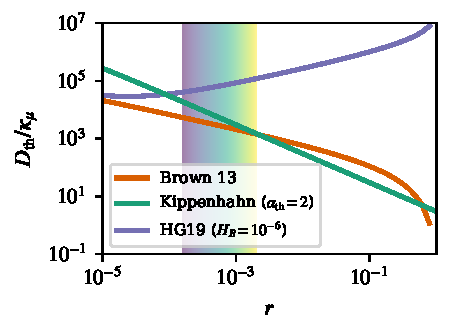
\includegraphics[width=\columnwidth]{Nu_models_comparison.pdf}
    \caption{ {\bf{(Done)}}
    Prescriptions of the compositional diffusivity due to thermohaline mixing $D_{\rm th}$ normalized by the molecular diffusivity $\kappa_{\mu}$ are plotted against the reduced density ratio $r$. For each prescription, we use $\mathrm{Pr} = \tau = 10^{-6}$, consistent with the conditions in these regions of RGB stars.
    We plot two hydrodynamic models, the \citet{brown_etal_2013} model (orange) and the \citet{kippenhahn_etal_1980} model with $\alpha_{\rm th} = 2$ (green). In both cases, the mixing efficiency decreases with $r$.
    The \citet{harrington} model (HG19) is also shown; it includes magnetic fields, which cause mixing efficiency to increase with $r$ for these parameters.
    The plotted curve for the HG19 model depends on $H_B$, which depends on the stellar structure and magnetic field strength; the plotted value is characteristic of the structure in the thermohaline zone of a 1.1 $M_\odot$ star at [Fe/H] = -0.2 with a magnetic field whose strength is $\mathcal{O}(100 \,\mathrm{G})$.
    The purple-to-yellow color gradient plotted in the background denotes the range of $r$ values that we measure in our grid of 1D stellar evolution models, which are displayed in Fig.~\ref{fig:mesa_r_spread}.
    }
    \label{fig:parameterization_compare}
\end{figure}




\section{Mixing predicted by 1D models}
\label{sec:mesa_models}
We use Modules for Experiments in Stellar Astrophysics
\citep[MESA][]{Paxton2011, Paxton2013, Paxton2015, Paxton2018, Paxton2019}.

https://www.overleaf.com/project/617b3cb8a0b9ee4a8f5db5fb
\section{1D calculations of stellar R0:Meridith}\label{sec:1D}
How is this done. math. any tricks related to extracting these things from MESA. averaging etc. cite previous work.

make plot of mass versus metallicity color coded by R0 at the RGB bump.


To make Adrian happy: run models and extract the fluid parameters at various time steps (onset of thermohaline, when thermohaline touches scz for the first time, all timesteps in between). How do the fluid parameters and change at these various timesteps. how do the ratios between different models depend on which timesteps you choose (hopefully not at all). Also run at different thermohaline proscriptions. Does that matter? Assuming it isn't grossly awful, proceed to the next step.





\section{Discussion}
\label{sec:discussion}
Thermohaline mixing has long been though to be a good candidate to explain the evolution of the surface chemistry of low-mass upper red giant branch stars. We show here that

\begin{itemize}
    \item mixing rates should strongly depend on the balance of (R0- redefine)
    
    \item stellar evolution models suggest that R0 should vary as a function of mass and metallicity. The real range covered in low-mass upper RGB stars is (a lot/ a little) compared to the range of simulations that have been done. These stellar evolution models suggest that R0 should depend strongly on composition and only weakly on stellar mass
    
    \item observations suggest that the amound of mixing is/is not strongly correlated with R0 as predicted in 3D. Observations indicate that as R0 increases, the mixing rate (increases/decreases) consistent with (cite simulations) but not (cite other simulations)
    
    \item this suggests that (things about 3D models)
    
    \item magnetized thermohaline is/is not a good predictive theory for mixing in low-mass upper RGB stars
\end{itemize}
    
    If this is the case, should use this theory to predict cool stuff for lithium rich star production, mass transfer systems, etc. 






\begin{comment}
%FIGURE omgcomp---------------------------------------------------
\begin{figure}[!htb]
\begin{center}
\includegraphics[width=9cm,clip=true, trim=0.5in 0in 0in 0in]{./Figs/protversusloggmodelpmmPYboth.eps}%[width=9cm, clip=true, trim=1in 1in 1in 1in]{./Figs/omgcomp.eps}
\caption{The measured core rotation rates for the stars in our sample as a function of gravity compared to the predictions of our solid body model (blue) and our model with a moderately differentially convection zone (pink), showing that these models provide limits on the allowable amount of radial differential rotation in the surface convection zone.}
%There seems to be some moderate evidence of core-envelope recoupling as the stars evolve on the secondary clump, although more measurements of evolved stars with slowly rotating surfaces would strengthen this conclusion.} %\textbf{mark a line for the selection effect?} }
\label{Fig:bothmodels}
\end{center}
\end{figure}
%FIGURE omgcomp---------------------------------------------------
\end{comment}

\begin{acknowledgements}

We thank C. Hayes, A. Jermyn, and M. Cantiello for helpful discussions that contributed to this work. 
 Support for this work was provided by NASA through the NASA Hubble Fellowship grant No.51424 awarded by the Space Telescope Science Institute, which is operated by the Association of Universities for Research in Astronomy, Inc., for NASA, under contract NAS5-26555.
 Computations were conducted with support from the NASA High End Computing (HEC) Program through the NASA Advanced Supercomputing (NAS) Division at Ames Research Center on Pleiades with allocation GID s2276 which is provided through NASA HTMS grant 80NSSC20K1280.



\end{acknowledgements}

\software{Astropy \citep{Astropy,Astropy_2018}, Matplotlib \citep{Matplotlib}, NumPy \citep{numpy}, SciPy \citep{2020SciPy-NMeth}}

\facilities{Du Pont (APOGEE), Sloan (APOGEE)} 

\bibliographystyle{aasjournal}
\bibliography{ms.bib, library.bib, library2.bib, thermohaline.bib, mesa.bib}


\appendix

\section{MESA}
\label{app:mesa}
The MESA EOS is a blend of the OPAL \citep{Rogers2002}, SCVH
\citep{Saumon1995}, FreeEOS \citep{Irwin2004}, HELM \citep{Timmes2000},
PC \citep{Potekhin2010}, and Skye \citep{Jermyn2021} EOSes.

Radiative opacities are primarily from OPAL \citep{Iglesias1993,
Iglesias1996}, with low-temperature data from \citet{Ferguson2005}
and the high-temperature, Compton-scattering dominated regime by
\citet{Poutanen2017}.  Electron conduction opacities are from
\citet{Cassisi2007}.

Nuclear reaction rates are from JINA REACLIB \citep{Cyburt2010}, NACRE \citep{Angulo1999} and
additional tabulated weak reaction rates \citet{Fuller1985, Oda1994,
Langanke2000}.  Screening is included via the prescription of \citet{Chugunov2007}.
Thermal neutrino loss rates are from \citet{Itoh1996}.

We create 1D stellar models and evolve them from the pre-main sequence until roughly the end of hydrogen shell burning.
We study stellar masses between 0.9 and 1.7 $M_{\odot}$ in steps of $0.2 M_{\odot}$.
We study metallicities [Fe/H] ranging from -1.4 to 0.4 in steps of 0.2.
To convert from metallicity units to MESA input $Y$ and $Z$ units, we assume a linear helium enrichment law \citep[per e.g.,][sec 3.1]{choi2016} where we assume a big-bang $Y_p = 0.2485$ and $\Delta Y / \Delta Z = 1.3426$ according to table 1 of \citet{tayar_etal_2022}.
The algorithm we use to calculate $X$, $Y$, and $Z$ from these values is identical to the one used in \url{https://github.com/aarondotter/initial_xa_calculator}; we use the opacity tables of \citet{GrevesseSauval1998} and [$\alpha$/Fe].
The specific [Fe/H] to ($X$, $Y$, $Z$) conversions used here are shown in table~\ref{table:feh_to_z}.

\begin{deluxetable}{c c c c}
\tablehead{
\colhead{[Fe/H]} & \colhead{$X$} & \colhead{$Y$} & \colhead{$Z$}
}
\decimals
\startdata
      0.400 & 0.66214302 & 0.29971262 & 0.03814436 \\
      0.200 & 0.69253197 & 0.28229599 & 0.02517204 \\
      0.000 & 0.71318414 & 0.27045974 & 0.01635613 \\
     -0.200 & 0.72686070 & 0.26262137 & 0.01051793 \\
     -0.400 & 0.73576323 & 0.25751912 & 0.00671765 \\
     -0.600 & 0.74149343 & 0.25423501 & 0.00427157 \\
     -0.800 & 0.74515509 & 0.25213642 & 0.00270849 \\
     -1.000 & 0.74748410 & 0.25080161 & 0.00171429 \\
     -1.200 & 0.74896112 & 0.24995509 & 0.00108379 \\
     -1.400 & 0.74989606 & 0.24941926 & 0.00068468
\enddata
\begin{caption}
    Mappings between $[$Fe/H$]$ values and MESA input values of $(X, Y, Z)$.
    \label{table:feh_to_z}
\end{caption}
\end{deluxetable}


{\color{red} Describe lines from inlist}

\subsection{Resolution testing}
We studied how varying the temporal and spatial resolution modifies the behavior of the thermohaline zone that develops between the burning shell and the convective envelop, and the results of these tests are summarized in TODO.
For the suite of simulations presented in this paper, we increased the spatial and temporal resolution of our simulations by using a mesh delta coefficient of 0.8 and time delta coefficient of 0.5 for most of the star's evolution.
After the main sequence once we measured $log g < 3$, we decreased the mesh delta coefficient to 0.5 and the time delta coefficient to 0.1; we found that this combination of temporal and spatial resolution produced high accuracy at reasonable computational cost.



\end{document}
